\documentclass[a4paper,12pt]{article}
\usepackage[labelfont=bf,font=small]{caption}


\usepackage{geometry}
\geometry{a4paper,left=25mm,top=25mm,right=25mm,bottom=25mm}

\usepackage[pdftex]{graphicx}
\usepackage{url}
% Only include extra packages if you really need them. Common packages are:
\usepackage{graphicx}	% Including figure files
\let\iint\relax
\let\iiint\relax
\let\iiiint\relax
\let\idotsint\relax
\usepackage{amsmath}
\usepackage{amssymb}

\usepackage{pdflscape}
\usepackage[utf8]{inputenc}
\usepackage{xfrac}
\usepackage{color}
\usepackage{rotating}
\usepackage{tabularx}


\usepackage{color}
\usepackage[dvipsnames]{xcolor}
\definecolor{mygray}{gray}{0.6}
\newcommand{\todo}[1]{\textcolor{red}{#1}}
\newcommand{\arxiv}{arXiv}


\usepackage[symbol]{footmisc}
\renewcommand{\thefootnote}{\fnsymbol{footnote}}
\usepackage{setspace}

\usepackage{lineno}
\linenumbers

\usepackage{amsmath}
%\usepackage[superscript,biblabel]{cite}

\usepackage[resetlabels,labeled]{multibib}
\newcites{main,method}{{},{}} 
\usepackage[superscript,nomove]{cite}

\usepackage{xpatch}
\newcommand\removebibheader
  {\@{}
    {\section*{}%
     \@{}{}%
    }{}{}{}%
  }

\title{The impact on academic productivity owing to the COVID-19 pandemic}

\author{Andrew R. Casey$^{1,2}$\footnote{andrew.casey@monash.edu},
        Ilya Mandel$^{1,2}$,
        Prasun K. Ray$^{3}$\\
\normalsize{$^{1}$School of Physics \& Astronomy, Monash University, Clayton 3800, Victoria, Australia}\\
\normalsize{$^{2}$Center of Excellence for Astrophysics in Three Dimensions (ASTRO-3D), Australia}\\
\normalsize{$^{3}$Department of Mathematics, Imperial College London, London, United Kingdom}
}

\renewcommand*{\thefootnote}{\arabic{footnote}}


% [X] Any figures missing?
% [X] Write about drop in physics.comp-ph and physics.soc-ph.
% [X] All figure captions, update any figures.
% [X] Quantify difference from model.
% [ ] Abstract
% [ ] Read-through and edit.
% [ ] Distribute for comment.


\date{}
\doublespacing
\begin{document}
\newpage
\setcounter{page}{1}
\resetlinenumber[1]

\maketitle


% Conclusions
% -> Most fields show no impact.
% -> Biggest negative impact is in fields where most research is presented at conferences, or experimental sub-fields.
% -> Condensed matter shows up-tick, where pre-prints have focussed on experimental design instead of experimental results.
% -> Biology has a peak, seems to be a lot of biologists posting to arxiv for the first time, or people contributing from other fields.


\noindent \textbf{`\emph{Publish or perish}' is an expression describing the pressure on academics to consistently publish research to ensure a successful career in academia. With a global pandemic that has changed the world, how has it changed academic productivity? Here we show that academics are collectively posting just as many publications as if there were no pandemic.
	% Here we show.
%	Here we show that academics are collectively posting just as many publications as if there were no pandemic. 
%	This remains true across nearly all fields of research, including those focussed on theoretical and experimental research.
%	The most significant change in academic publishing is seen in biology, where there was a doubling of pre-prints posted in 2020. 
%	However, most of these extra pre-prints are not written by, or with, biologists.
%	\todo{At least half} of the excess biology pre-prints are entirely authored by researchers from other fields, primarily physicists.
%	No broad impact is found between theoretical and experimental research.
%	Reduced access to experimental laboratories seems to have motivated researchers to publish more papers (overall) based on work that was already in preparation. The full impact of the pandemic on academic publishing may not yet be fully realised.	
%	Many fields undeterred; posting just as many as before.
%	Some fields show a large increase (q-bio),
%	Others, mostly experimental fields, show a marked decline in preprints.
}\\


%----------------------------------------------------------------------------------------
%	MAIN MATTER OF THE DOCUMENT
%----------------------------------------------------------------------------------------

\noindent Peer-reviewed publications are the most common measure of productivity in academia. The \arxiv\cite{Ginsparg:2011} ({https://arxiv.org}) is a distribution service for research publications before they are printed in a journal (i.e., a pre-print). A pre-print on \arxiv\ does not ensure that the contents have passed peer-review, but most material on \arxiv\ eventually goes through peer-review because it is now standard in many research fields to post to \arxiv\ either during or after the peer-review process \cite{Lariviere:2014}. For this reason, the number of pre-prints posted to \arxiv\ approximates the number of peer-reviewed publications written at any time.


Here we make quantitative comparisons on the number of pre-prints posted to \arxiv\ before and during the pandemic. While we investigate the impact that the COVID-19 pandemic has had on different fields of research, we highlight that we are unable to identify or differentiate between authors and communities whose productivity has been significantly harmed by the pandemic, and those who were largely unscathed. The COVID-19 pandemic has impacted the population in unequal ways\cite{Nicola:2020,Chu:2020,IbnMohammed:2021}. Generational inequality, career stage, personal circumstances, carer responsibilities, work environments, places of employment, and many other factors, all significantly contribute to the disproportionate and unequal impact the pandemic may have had on a scientist's capacity to conduct research. 
%These factors are more important determinants to research capacity than a scientist's field of research. 
While this limited analysis does not address these issues, it is important to consider that while a community as a whole has not yet demonstrated a significant change in productivity, many researchers have faced significant challenges and suffered physically, mentally, emotionally, and professionally. 


We retrieved metadata for 1,475,914 pre-prints posted on the \arxiv\ between 1 April 2007 and 31 May 2021. The metadata includes the creation date, research field(s), title, author name(s), abstract, and other miscellaneous information\cite{Clement:2019}. There is an increasing number of pre-prints posted to \arxiv\ each year in nearly every field (Figure~1). These long-term trends are relatively predictable from year to year, allowing us to quantify any change in academic productivity due to the COVID-19 pandemic. We used the number of publications from January 2008 to December 2019 to predict the expected number of monthly pre-prints in 2020 in each field. We modelled the number of monthly pre-prints in each field using a Gaussian Process with a quasi-periodic kernel function\cite{Rasmussen:2006,Ambikasaran:2014}, allowing us to accurately predict long-term trends and periodicity in given fields of research (Figure~1). In nearly all research fields the number of pre-prints posted since January 2020 agree excellently with the model predictions, indicating no collective impact (positive or negative) on academic productivity due to the COVID-19 pandemic.

\noindent\todo{Include a table with each field where we quantify the change?}
% field     & 2020 pre-prints & YoY change from 2019 to 2020 & Predicted pre-prints in 2020 & Number of sigma deviations away from model
%astro-ph    & 14,893    &  +3.4 & 14,948 \pm 655    & -0.1 
%cond-mat    & 16,188    &  +7.0 & 15,098 \pm 544    & +2.0 
%cs          & 54,808    & +24.3 & 50,567 \pm 3153   & +1.3 
%gr-qc       & 3,405     & +12.4 & 3,178 \pm 202     & +1.1 
%hep-ex      & 615       & -19.8 & 797 \pm 131       & -1.4 
%hep-lat     & 394       & -19.3 & 474 \pm 185       & -0.4 
%hep-ph      & 4,586     &  +1.3 & 4,563 \pm 285     & +0.1 
%hep-th      & 3,869     &  +0.9 & 3,971 \pm 262     & -0.4 
%math        & 35,367    &  +5.5 & 35,409 \pm 1974   & -0.0 
%math-ph     & 1,378     &  -6.3 & 1,445 \pm 131     & -0.5 
%nlin        & 885       &  +6.1 & 820 \pm 64        & +1.0 
%nucl-ex     & 499       &  +2.9 & 479 \pm 62        & +0.3 
%nucl-th     & 1,212     &  -3.2 & 1,248 \pm 97      & -0.4 
%physics     & 15,241    & +14.3 & 14,612 \pm 959    & +0.7 
%q-bio       & 2,790     & +49.0 & 1,944 \pm 191     & +4.4 
%q-fin       & 979       & +23.1 & 812 \pm 74        & +2.3 
%quant-ph    & 6,341     & +13.4 & 6,210 \pm 269     & +0.5 
%stat        & 5,180     & +20.2 & 4,719 \pm 509     & +0.9 


Border closures and travel restrictions have forced many academic conferences to be held online-only, or to be cancelled. The immediate impact of cancelling a conference is readily apparent in pre-print counts in lattice physics (Figure~1; \arxiv\ subject code \texttt{hep-lat}, see Methods for explanation), where most pre-prints are posted around December each year as conference proceedings from the International Symposium on Lattice Field Theory. In 2020 the conference was cancelled\cite{LatticeConferenceWebsite} and no accompanying pre-prints exist. However, the impact on research from travel restrictions is likely to be much longer than what is represented by the drop in lattice physics pre-prints. Discussions at conferences or collaborative visits frequently spark new research ideas that might lead to a publication many months or years later. 
% TODO: Consider moving this paragraph elsewhere to better align with the long timelines of research.

Experimental research projects often require specialised laboratories, or data to be collected over many years. The pandemic has forced many laboratories to close or operate with restricted access, which could lead to long-lasting delays in ongoing experiments or immediate drops in publication rates in part due to difficulty in accessing completed (or nearly completed) experiment data. There is some evidence of this in pre-print numbers already, with {25\%} fewer pre-prints in high energy physics (\texttt{hep-ex}) in 2020 than expected by our model (observed 615; predicted 797 $\pm$ 131). But declines are not ubiquitous across experimental fields. The closest comparable field of phenomenology in high energy physics (\texttt{hep-ph}) showed no decline. And throughout 2020, experimental research in condensed matter (\texttt{cond-mat}) saw a 2$\sigma$ increase above our model predictions (observed 16,188; predicted 15,098 $\pm$ 544). Segmenting condensed matter pre-prints by research topic shows that most of this increase (in \texttt{cond-mat}) was driven by a 30\% increase in material science pre-prints (\texttt{cond-mat.mtrl-sci}), a sub-field of condensed matter that focusses on laboratory methods and techniques. Despite the COVID-19 pandemic restricting access to essential laboratory equipment, this shift to publish methods and experimental design work -- which might otherwise be neglected due to ongoing laboratory work -- produced an immediate boost in condensed matter research. This is likely an effect with a limited lifespan: eventually, condensed matter (and other experimental) research will require laboratory access to continue publishing.

The field of quantitative biology (\texttt{q-bio}) research showed the largest increase in pre-prints in 2020 above what is expected by our model. There were {2,790} quantitative biology pre-prints in 2020, {50\%} above the previous year, representing a $+4.4\sigma$ deviation from our model predictions (predicted 1,944 $\pm$ 191). This increase is explainable by an increase in COVID-19 related research, as there were 844 quantitative biology pre-prints in 2020 with pandemic-related terms in their title or abstract (see Methods), and just 43 in the decade prior. Indeed, in {April 2020} nearly 60\% of the \arxiv\ pre-prints in quantitative biology were related to the pandemic (Figure~2). Pandemic-related pre-prints also appeared in other fields (computer science, physics, statistics, and quantitative finance, all peaking around {April 2020}, but pandemic-related pre-prints constituted less than 10\% of the pre-prints in these fields. As of mid-2021 the number of monthly pre-prints in quantitative biology has dropped to pre-pandemic levels, although approximately 20\% of these pre-prints are related to the ongoing pandemic, representing a strong shift in ongoing research focus.
 
 
An increase in quantitative biology\footnote{Quantitative biology is only a sub-field of biology, and most biology pre-prints are posted to bioRxiv ({https://biorxiv.org}).} research during a global pandemic is unsurprising. However, the \arxiv\ data shows that this increase in pre-prints was not driven by biology researchers posting twice as many pre-prints than usual. In 2020 there was a peak in the number of new authors appearing for the first time in the quantitative biology literature (Figure~3) while the number of new authors in all other fields remained steady. The sudden influx of new authors cannot be explained by large ($>$10) newly-formed collaborations working together to tackle the impending pandemic (Figure~4). The increase in pre-prints (and new authors) is driven by small (1-4) groups of authors, where many had never posted pre-prints to quantitative biology before.


Some of these new authors in quantitative biology have never before appeared in any other \arxiv\ fields, either.
A close examination of these pre-prints reveals that many are established biologists who have not used the \arxiv\ before, and are now doing so presumably to help ensure that their COVID-19 research is more widely available. This represents a genuine increase in new researchers to the \arxiv, and a boost to making quantitative biology research more widely accessible. Of those new authors in quantitative biology who also appear in other \arxiv\ fields, some of this will be due to name confusion (see Methods): where two researchers in different fields share the same publishing name. However, a careful examination of pandemic-related pre-prints in quantitative biology that were posted in 2020 shows that many were indeed written by researchers from other fields (primarily physicists and mathematicians), who had never before posted about quantitative biology. These pre-prints tend to focus on modelling the COVID-19 outbreak using public data sets, rather than quantitative biology research that requires more expert domain knowledge. 


%Any contributions by physicists or mathematicians to quantitative biology did not lead to significant drops in pre-prints in physics or maths. Throughout 2020 there were just as many pre-prints posted in physics as our model predicts, but an unusual asymmetry is present: with more pre-prints posted in the first half of 2020 than those in the later half. Other fields show strong seasonality in pre-prints (e.g., \texttt{hep-lat}), but physics does not. This seasonality in 2020 physics pre-prints is also conflated by a some physics sub-fields that saw a short burst of increased productivity early in 2020, before the effects of the pandemic were widespread (Figure~5). 


%drastic drop in productivity (Figure~5). Specifically, pre-prints in computational physics (\texttt{physics.comp-ph}) and \emph{Physics and Society} (\texttt{physics.soc-ph}) peaked to their highest level in \todo{March 2020} before declining rapidly to levels not seen since 2018. 

% -> timescales.

The COVID-19 pandemic has had disparate impacts on research productivity in different fields. Some fields show a drop in research outputs. Few show an increase, either driven by pandemic-related research or by shifts away from experimental research to topics that do not require ongoing laboratory access. In this study we have only focussed on quantity of publications as a measure for productivity, and not their quality. While citations are the most commonly used measure of impact of academic publications, that metric becomes a more biased statistic when many related pre-prints are all being posted nearly at the same time. 
The relatively long timescales of academic research would suggest that the full impact on academic productivity due to the COVID-19 pandemic is yet to be seen. For those fields without a measurable drop in research outputs yet, it's plausible that many of the pre-prints being posted are research projects that were well underway before the pandemic, with the full impact of academic research yet to be seen.


%Even among the measurable changes that we have discussed, none have fully returned to normality: even while quantitative biology pre-prints have returned to pre-pandemic levels, 20\% of the research in that field is now related to the ongoing pandemic. 



%----------------------------------------------------------------------------------------
%	References
%----------------------------------------------------------------------------------------

%\bibliographystylemain{myieeetr2}

%\vspace{-4cm}
%\bibliographyNew{references_new.bib}
%{\removebibheader
 %\bibliographymain{references_new.bib}
%}

%\bibitem{Papics2017}
%{P{\'a}pics}, P.~I., {\em et~al.}, {Signatures of internal rotation discovered
%  in the Kepler data of five slowly pulsating B stars}, {\em \textit{Astron.
%  Astrophys.}}, {\bfseries 598}, A74, 2017.

\begin{thebibliography}{10}

\bibitem{Ginsparg:2011}
{Ginsparg}. P., {ArXiv at 20}, \emph{Nature}, \textbf{476}, 7359, doi:10.1038/476145a \newblock (2011).

\bibitem{Clement:2019}
{Clement, C.~B., Bierbaum, M., O'Keeffe, K.~P., Alemi, A.~A.,}
{On the Use of ArXiv as a Dataset},
Preprint at https://arxiv.org/abs/1905.00075 \newblock (2019).

\bibitem{Lariviere:2014}
%{Larivi{\'e}re, V., Sugimoto, C.~R., Macaluso, B., Milojevi{\'c}, S., Cronin, B., Thelwall, M.,} 
{Larivi{\'e}re, V., et al.,} {arXiv E-prints and the journal of record: An analysis of roles and relationships}, \emph{Journal of the Association for Information Science and Technology}, \textbf{65}, 6, doi:10.1002/asi.23044 \newblock (2014).

\bibitem{IbnMohammed:2021}
{Ibn-Mohammed, T., et al.,} {A critical analysis of the impacts of {COVID}-19 on the global economy and ecosystems and opportunities for circular economy strategies}, \emph{Resources, Conservation and Recycling}, \textbf{164}, 105169, doi:1016/j.resconrec.2020.105169 \newblock (2021).

\bibitem{Nicola:2020}
{Nicola, M., et al.,} {The socio-economic implications of the coronavirus pandemic ({COVID}-19): A review}, \emph{International Journal of Surgery}, \textbf{78}, 185--193, doi:10.1016/j.ijsu.2020.04.018 \newblock (2020).

\bibitem{Chu:2020}
{Yen-Hao Chu, I., Prima, A., Larson, H.~J., Leesa, L.}
{Social consequences of mass quarantine during epidemics: a systematic review with implications for the {COVID}-19 response}, \emph{Journal of Travel Medicine}, \textbf{27}, 7, doi:10.1093/jtm/taaa192 \newblock (2020).


\bibitem{Rasmussen:2006}
{Rasmussen, C.~E., Williams, C.~K.~I.,}
{Gaussian Processes for Machine Learning}, \emph{MIT Press}, ISBN 026218253X \newblock (2016).

\bibitem{Ambikasaran:2014}
{Ambikasaran, S., Foreman-Mackey, D., Greengard, L., Hogg, D.~W., O'Neil, M.,}
{Fast Direct Methods for Gaussian Processes}, Preprint at http://arxiv.org/abs/1403.6015 \newblock (2014).
 
\bibitem{LatticeConferenceWebsite}
Helmholtz-Institut f\"ur Strahlen- und Kernphysik Indico Service (Indico). 2021. \emph{The 38th International Symposium on Lattice Field Theory (Lattice 2020)}. [online] Available at: {https://indico.hiskp.uni-bonn.de/event/1/} [Accessed 3 June 2021].


%\bibitem{kippenhahn2012}
%{Kippenhahn}, R., {Weigert}, A., and {Weiss}, A., {\em {Stellar Structure and
%  Evolution, Astronomy and Astrophysics Library, Springer Berlin Heidelberg}}.
%\newblock 2012.


\end{thebibliography}

%\end{document}
\newpage
%----------------------------------------------------------------------------------------
%	Figures
%----------------------------------------------------------------------------------------
\begin{center}
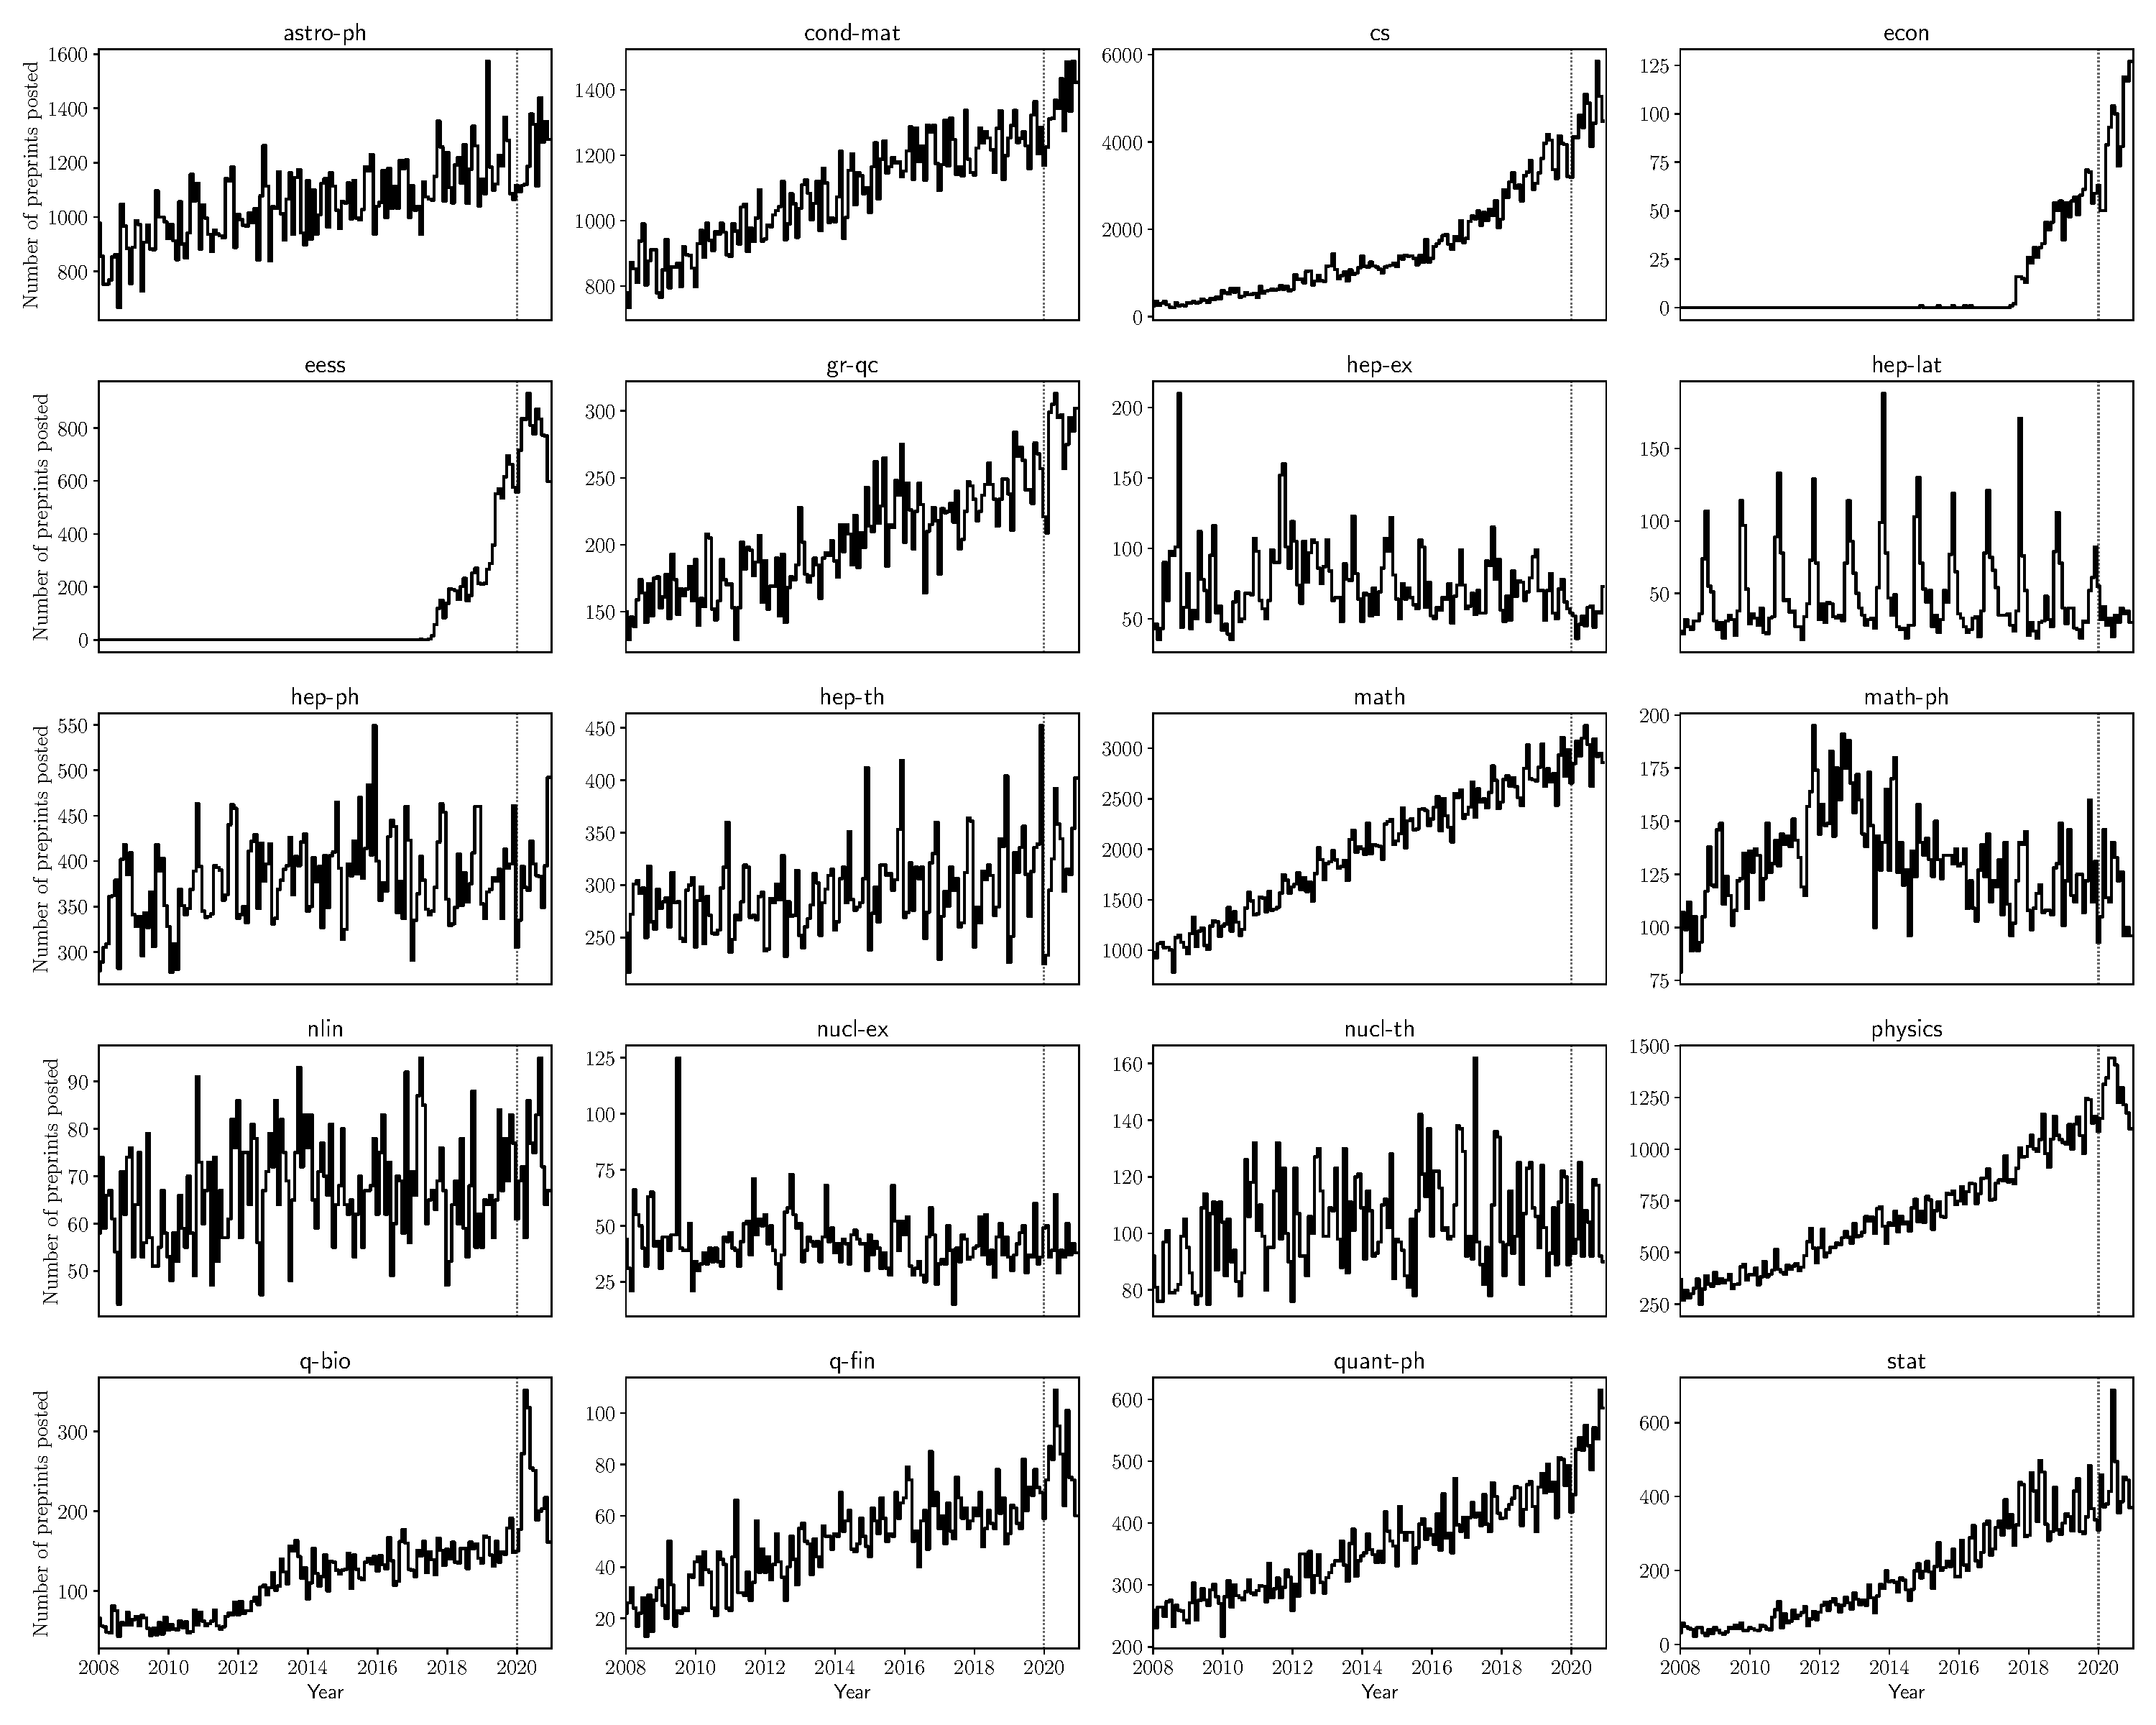
\includegraphics[width=0.95\linewidth]{pre-prints-segmented-by-field}
\end{center}

\noindent \textbf{Figure 1:} \textbf{Since the COVID-19 pandemic began there has been no significant change in monthly \arxiv\ pre-prints in most fields (black).} The expected number of pre-prints from our model is shown in red, and the red region shows the uncertainty in that expectation. Each panel shows a primary field of research in \arxiv. \todo{Blue is ARIMA model.}

\newpage

\begin{center}
 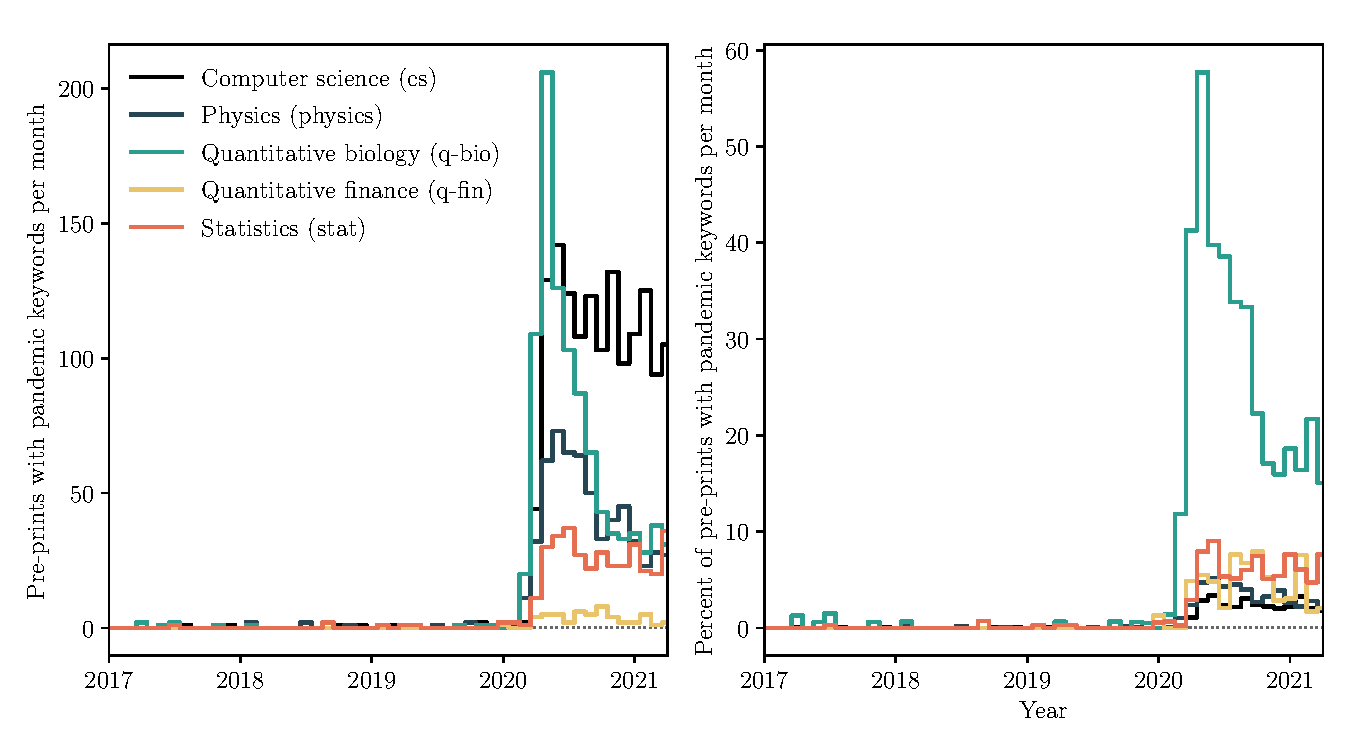
\includegraphics[width=\linewidth]{pandemic-related-preprints.pdf}
\end{center}

\noindent \textbf{Figure 2: Pre-prints related to the COVID-19 pandemic peaked in quantitative biology in 2020, accounting for nearly 60\% of quantitative biology pre-prints.} Shown are five other research fields with the highest number of pandemic-related pre-prints in 2020. Monthly pre-prints are shown on the left, and the percent of pandemic-related pre-prints in that research field is shown on the right.

\newpage

\begin{center}
	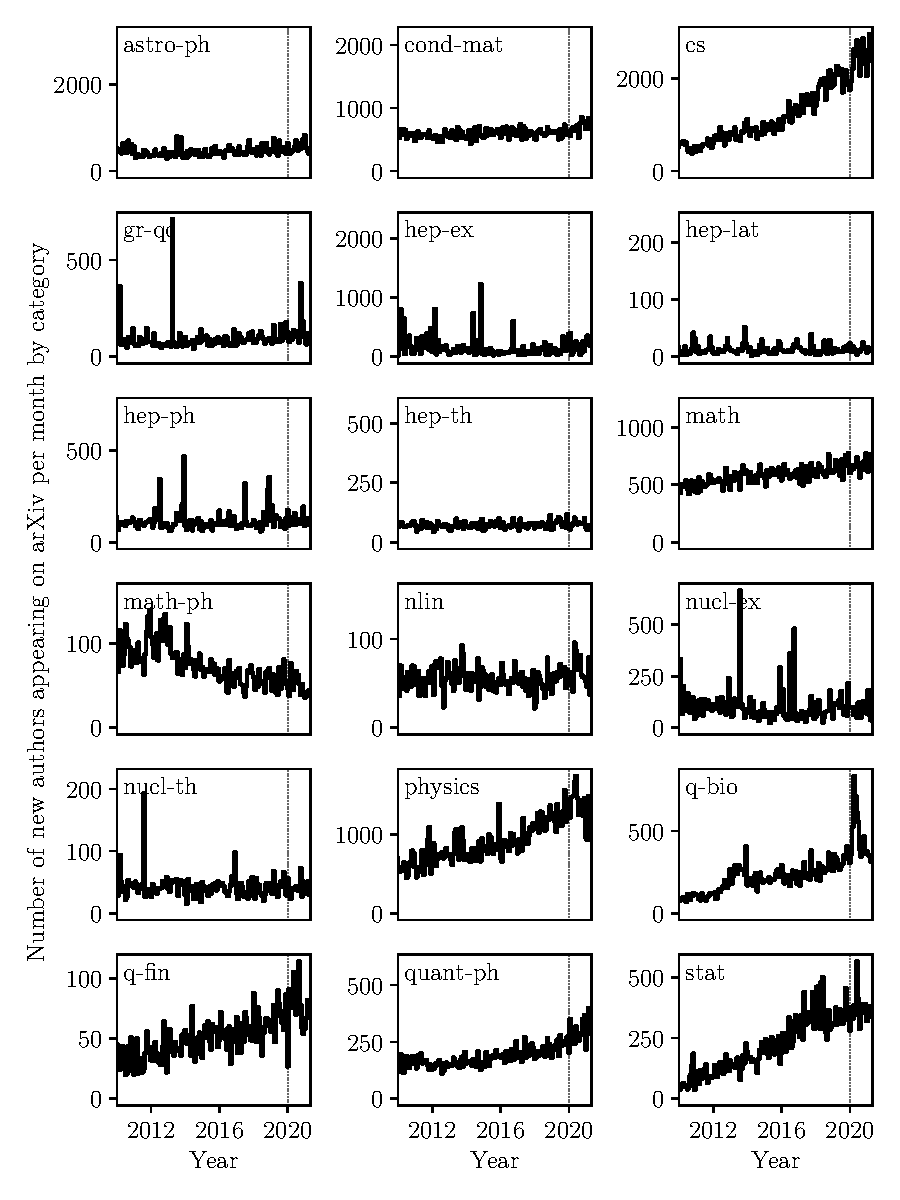
\includegraphics[width=0.95\linewidth]{new-authors-segmented-by-field}
\end{center}

\noindent \textbf{Figure 3:} \textbf{The number of new authors appearing in \arxiv\ pre-prints per month peaked in quantitative biology in 2020.} Fields well-established before 2007 (e.g., \texttt{astro-ph}) show an apparent influx of `new authors' at the time the data starts: these authors are already established academics. The slow change in new authors after 2012 approximates the net number of new authors joining the field.

\newpage


\begin{center}
     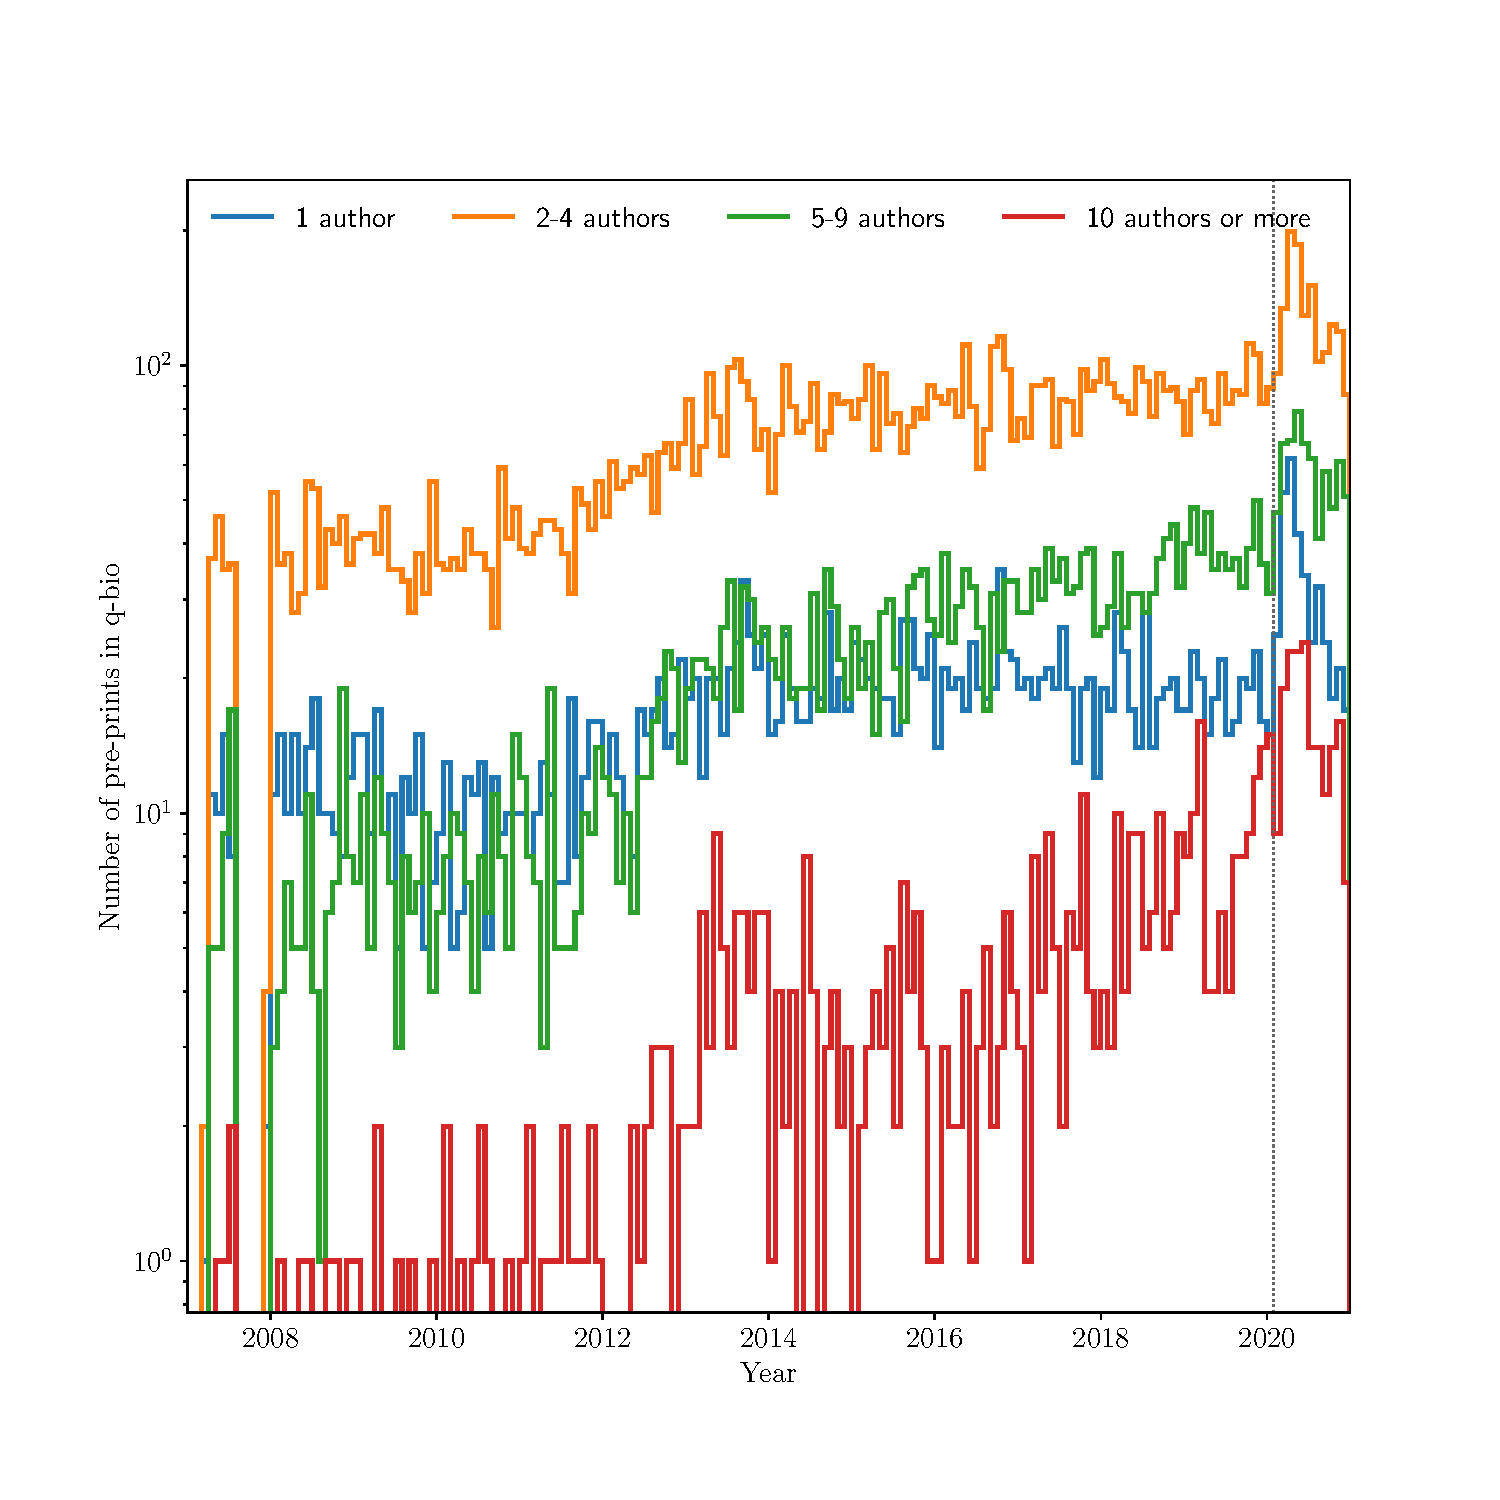
\includegraphics[width=\linewidth]{q-bio-pre-prints-segmented-by-author-count}
\end{center}

\noindent \textbf{Figure 4:} \textbf{The increase in quantitative biology pre-prints in 2020 cannot be attributed to large collaborations.} The coloured regions represent the different author group sizes for quantitative biology pre-prints per month with time.


\newpage

%\begin{center}
%     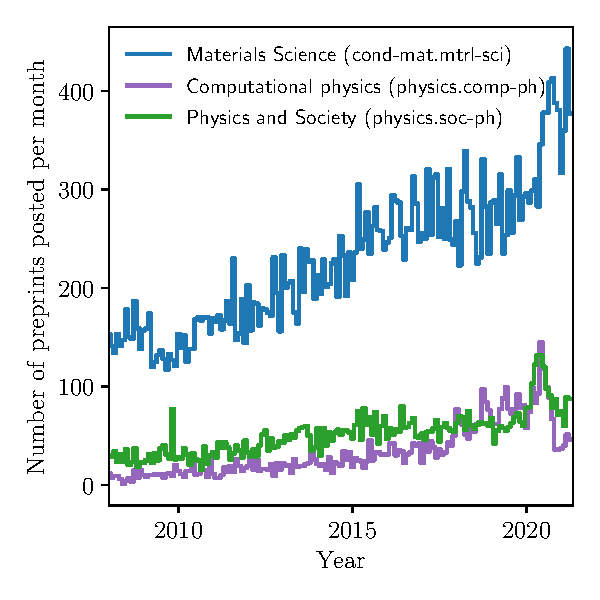
\includegraphics[width=\linewidth]{winners-and-losers-of-covid}
%\end{center}

%\noindent \textbf{Figure 5:} \textbf{Mat-sci}


\newpage
%----------------------------------------------------------------------------------------
%	Methods
%----------------------------------------------------------------------------------------
\section*{Methods}


\subsection*{Long-term modelling of monthly pre-print counts}

We use monthly pre-print counts per primary research field from January 2007 until December 2019 to make predictions for the number of pre-prints expected per month from January 2020 onwards. We use a Gaussian process with a quasi-periodic kernel covariance function to model long-term trends and seasonal periodicity\cite{Rasmussen:2006,Ambikasaran:2014}. We fix the periodicity hyper-parameter to one year, and optimise all other hyper-parameters. The predictions of the expectation and variance in the number of monthly pre-print counts are conditioned on the optimized hyper-parameters. We fit this model to monthly pre-print counts for every primary research field.

\todo{We also considered an ARIMA model. The results were very similar. The largest difference between predictions is in \texttt{quant-ph}. Conclusions remained the same. Happy to use either, although I think a Gaussian process (which here is similar enough to a Poisson process) is a closer approximation to the data generating process.}

\subsection*{Segmenting by research field}

Pre-prints posted to the \arxiv\ can be listed in a single field of research, or cross-listed in multiple fields. A field is annotated by \texttt{primary.SEC} where the primary field of research has the prefix, and the sub-field of research is represented by a short capitalised suffix. For example, one pre-print may have a primary field of research as stellar astrophysics (\texttt{astro-ph.SA}) and be cross-listed in machine learning (\texttt{stat.ML}). These field(s) of research are supplied by the corresponding author. It is a subjective decision whether to include more than one field of research, or what those fields of research would be. For this reason, throughout this work when we segment by research field we take the primary parent research field provided and ignore any cross-listed fields of research. When we segment pre-prints by sub-field, we similarly take the primary sub-field provided and ignore any cross-listings.


\subsection*{Uniquely identifying authors}

The \arxiv\ metadata available to us does not include institutional affiliations, or identifiers that would uniquely identify an author. For these reasons, we have taken steps to minimise the effects of name confusion. There are two primary ways that name confusion could impact our inferences. In the first scenario, two people with the same name are amalgamated and treated as a single author that is on average twice as productive (or more, for very common names) as other authors. In the second scenario, an author will sometimes publish as `A.~B.~Smith', and other times publish as `A.~Smith'. A careful exploration of the data shows that this is a very frequent scenario, and if left uncorrected, would appear as many `unique' authors with half as many publications on average.

We have taken a simple approach to address name confusion. We first define a unique author by family name and the initial of the first given name (`Family-name, I.'), such that we intentionally group together authors that may share the same initial of their second given name. While our approach to name confusion is grossly simple, it is unlikely that these choices have any substantial impact on our inferences. Any common name is likely to appear in the literature early in the data set, and will not impact the conclusions we draw about how publishing changed in 2020. 
%While common names will appear between different fields (e.g., quantitative biology and physics), by showing this as a function of time we get an intrinsic measure of the name ambiguity between fields, and we see the increase in overlap when a spike in quantitative biology papers occurs. 
%Nevertheless, we manually inspected horiz of quantitative biology pre-prints that entirely consisted of `new authors' and cross-referenced these with Google Scholar to confirm that these authors were established researchers in other fields, and not biologists posting pre-prints for the first time.

\subsection*{Pre-prints related to the COVID-19 pandemic}

We identified a pre-print as being related to the COVID-19 pandemic if the title or abstract contained any of the following four (case-insensitive) terms: `pandemic', `COVID', `SARS-CoV-2', or `lockdown'. Before 2020, these terms rarely appear in the title or abstract of any pre-print on \arxiv\ (Figure~2).

%----------------------------------------------------------------------------------------
%	Data availability
%----------------------------------------------------------------------------------------

\section*{Data availability}

The entire dataset used in this article is from \arxiv. The dataset is curated by Cornell University and hosted by Kaggle (https://www.kaggle.com/Cornell-University/arxiv). We accessed this dataset on 01 June 2020.

%This data set includes the identifier and metadata for all pre-prints posted to \arxiv, and is updated weekly. 
%A pre-print's identifier is defined by the year and month that the pre-print was posted, and the number of pre-prints already posted in that month (across all fields). For each pre-print the metadata includes  the title, author name(s), abstract, research field(s), and the date the pre-print was first posted. Pre-prints posted prior to 2007 use a different identifier scheme, and for this reason we have excluded pre-prints earlier than this date. The data set used for analysis includes \todo{1,379,332} pre-prints posted between \todo{2007-03-30} and \todo{2020-12-30}.

%All data was sourced from Kaggle (https://www.kaggle.com/Cornell-University/arxiv) on 1 June 2020.

\section*{Code availability}
The software developed to retrieve and analyse the data for this projectis available online (https://github.com/andycasey/arxiv-covid).


%----------------------------------------------------------------------------------------
%	Methods references
%----------------------------------------------------------------------------------------


%----------------------------------------------------------------------------------------
%	Acknowledgements
%----------------------------------------------------------------------------------------
\section*{Acknowledgements}
We thank Peter Skands (Monash University) 
	 and Ross Young (University of Adelaide) 
for comments on publication trends in high energy physics.


%----------------------------------------------------------------------------------------
%	Author contributions
%----------------------------------------------------------------------------------------

\section*{Author contributions}

All authors contributed to the discussions and have read and iterated upon the text of the final manuscript. 

%----------------------------------------------------------------------------------------
%	Competing interests
%----------------------------------------------------------------------------------------
\section*{Competing interests}
The authors declare no competing interests. 

%----------------------------------------------------------------------------------------
%	Materials and correspondence
%----------------------------------------------------------------------------------------
\section*{Materials \& Correspondence}
Correspondence and requests for materials should be addressed to the corresponding author Andrew Casey (andrew.casey@monash.edu).

%----------------------------------------------------------------------------------------
%	Additional information
%----------------------------------------------------------------------------------------
\section*{Additional information}

\textbf{Supplementary Information} is available for this paper.

\noindent\textbf{Correspondence and requests for materials} should be addressed to A.~R.~C.

\noindent\textbf{Reprints and permissions information} is available at {\tt\small www.nature.com/reprints}

\end{document}
